\section{数据理解与总体分析}
\subsection{数据处理与评价区间}
附件1给出144个10分钟时段的典型日电价、负荷和光伏；附件2给出2025年实际负荷与光伏；附件3给出每天四次发布的24小时光伏预报；附件4给出波动电价。本文以电量为优化变量，功率乘$\Delta t=1/6$小时后统一为kWh，电价保持元/kWh。
附件与结果模板的时间文字存在一个10分钟刻度差异，因此输出沿用模板标签，以行列序号一一对应原始槽数据，避免因字符串匹配造成错位。本文指定时段表也沿用结果模板标签。

附件3中提前$k$小时的值对应发布时刻加$k$小时，故每次更新都按发布时刻重建时间轴，再插值至10分钟粒度。6、12、18时预报只用于该次发布之后尚未执行的时段，不能直接套用零点预报的映射。
负荷与光伏历史预测均仅使用决策日前的实际值；典型日曲线视为题目给定的外生参考资料，不从完整年度实际值重新计算。

根据结果模板，问题二至四统一评价2025年2月1日至12月31日，共334天。1月数据用于形成滞后特征与预热权重。当前实验在2月1日以6000 kWh初始化储能；这是评价区间的统一初始条件，并非对1月运行后的储电量进行推导。题面给出1月1日初值，因此本文结果应理解为指定报送区间的条件回测，初始状态的局限在模型评价中讨论。

\subsection{误差结构与决策目标}
数据分析表明，光伏光照样本的预测误差随提前时间增加，近似关系为
$\mathrm{MAE}(k)\approx14.8+29.0k$ kW，拟合$R^2=0.982$。
下午13至18时的光伏MAE随发布时刻由零点推进至6时、12时，从413 kW降至248 kW、76 kW。
日内误差的前四阶相关系数为0.79、0.60、0.40、0.21，说明逐点独立扰动会破坏误差的时间结构。
因此，日内更新预报具有调度价值；整日联合残差场景作为候选扩展，通过消融决定是否进入正式方案。

紧急购电与计划购电的价格不对称，最小预测均方误差并不直接等于最小购电成本。
本文用历史实现费用标定预测组合，在名义预测上加入小幅保守修正，再利用当前实际状态逐槽执行。
候选场景法保留负荷和光伏残差的同日联合结构，避免只考虑光伏误差而遗漏净负荷风险；若留出实验不支持，则按简约原则删除。

\subsection{两日规划与滚动执行}
每天零点优化当日与次日共288个槽，只承诺首日计划；次日计划是储能机会成本的近似参考，到次日零点会重新计算。该思路借鉴滚动时域优化\cite{mayne2000}，但本文采用的有限窗口与实时执行规则并不具有自动成立的无限时域最优性保证。
问题三在日内预报发布时重算剩余时段，执行层每10分钟只读取当前实际值，日末储电量自然传递至次日。
表\ref{tab:info}概括不同问题的信息范围。
\begin{table}[htbp]\centering
\caption{各问题的信息集与调度结构}\label{tab:info}
\small
\begin{tabularx}{\textwidth}{c X X X}
\toprule
问题 & 零点负荷与光伏输入 & 电价输入 & 调整与储能结构\\
\midrule
一 & 典型日给定数据 & 典型日给定 & 单日规划、日循环\\
二 & 因果历史预测 & 典型日电价 & 无日内调整、两日滚动\\
三 & 历史负荷与组合光伏预报 & 典型日电价 & 三次更新、跨日连续\\
四 & 分别沿用问题二、三预测 & 给定波动电价G & 分别重算两层策略\\
扩展H & 与问题四对应层一致 & 历史价格预测 & 评价电价信息价值\\
\bottomrule
\end{tabularx}
\end{table}

\subsection{统一求解框架}
四问共用同一套“预测—计划—调整—执行—结算”框架，仅在题面允许的信息集与结算目标上存在差异。
图\ref{fig:corealg}给出该统一核心算法：每天零点先用决策日前的实际值构造负荷与光伏的自适应组合预测
（问题三、四在光伏上另与官方预报组合），权重按历史实现费用以指数加权方式逐日标定；
对预测施加负荷抬升与光伏折减的保守裕度后，求解当日与次日共288个槽的购电与储能线性规划，
规划窗口末端自由，只承诺首日计划。问题三与问题四在6、12、18时以最新发布的预报和当时的
实际储电量重算剩余时段，调整量按调低部分付50\%、调高部分付150\%的规则产生偏差费用；
执行层逐槽读取当前已实现的负荷与光伏，缺口按当期电价5倍紧急购电，富余只能弃光，
日末储电量自然传递至次日并触发滚动重解。问题一为确定性特例，采用单日循环模型；
问题四仅将价格输入替换为附件4的波动电价。图中每一环节的“口径”行汇总了对应问题的信息集差异。
\begin{figure}[htbp]\centering
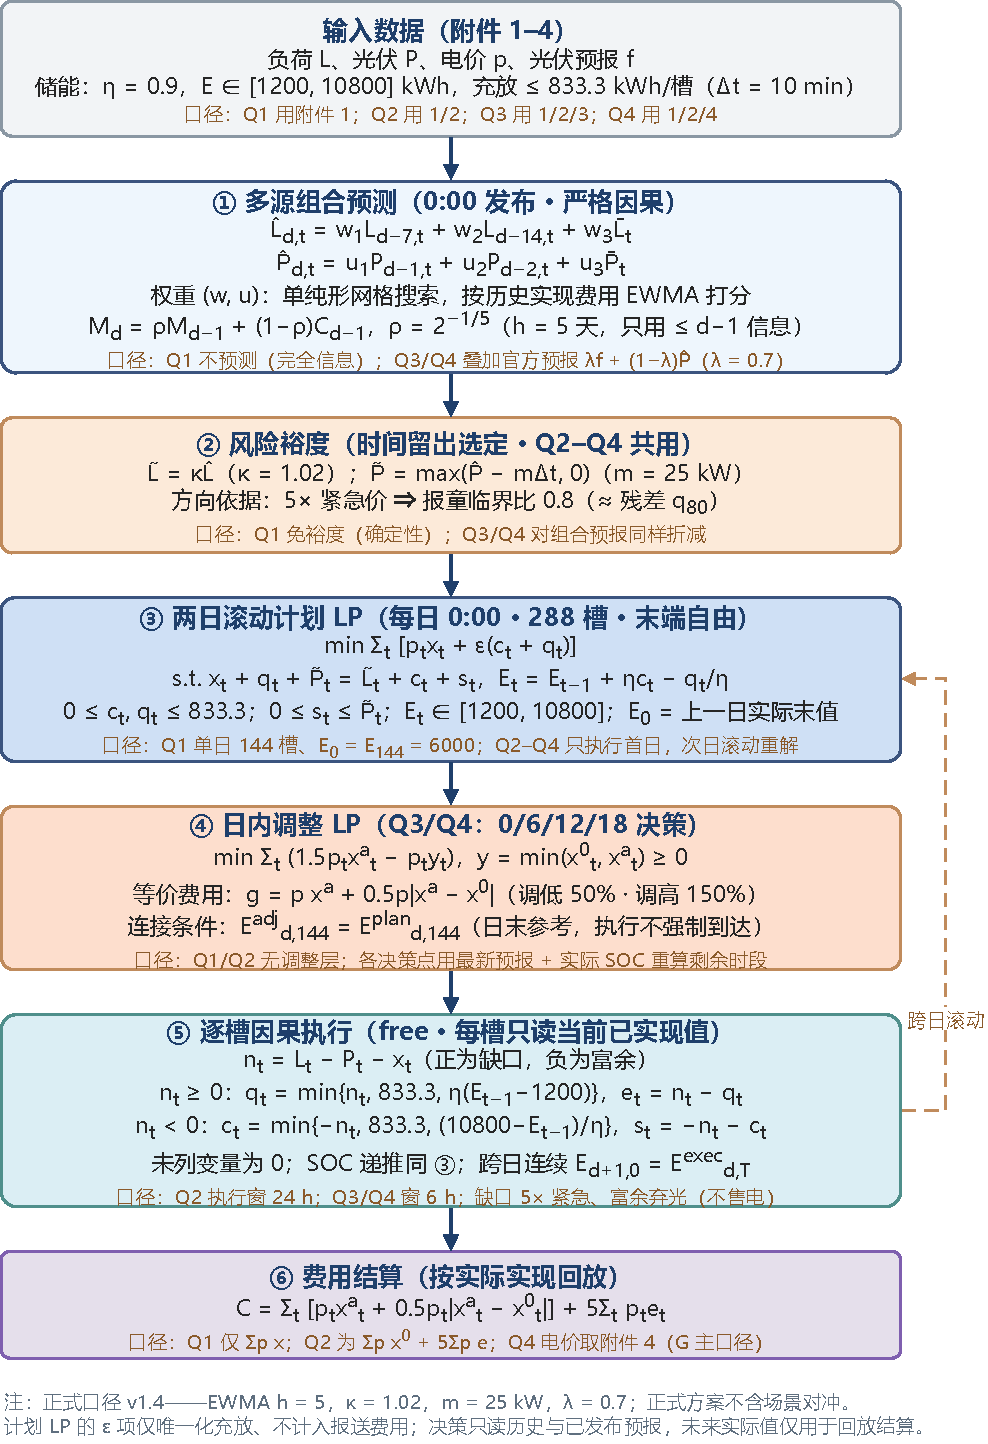
\includegraphics[width=.9\textwidth]{../../figures/核心算法流程图.pdf}
\caption{Q1--Q4共用的统一核心算法流程（含各问信息集差异与结算口径）}\label{fig:corealg}
\end{figure}
